
%%%%%%%%%%%%%%%%%%%%%%%%%%%%%%%%%%%%%%%%%%%%%%%%%%%%%%%%%%%%%%%%%%%%%%%%%%%%%%%%%%%%%%%
%%%%%%%%%%%%%%%%%%%%%%%%%%%%%%%%%%%%%%%%%%%%%%%%%%%%%%%%%%%%%%%%%%%%%%%%%%%%%%%%%%%%%%%
% 
% This top part of the document is called the 'preamble'.  Modify it with caution!
%
% The real document starts below where it says 'The main document starts here'.

\documentclass[12pt]{article}

\usepackage{amssymb,amsmath,amsthm}
\usepackage[top=1in, bottom=1in, left=1.25in, right=1.25in]{geometry}
\usepackage{fancyhdr}
\usepackage{enumerate}
\usepackage{listings}
\usepackage{graphicx}
\usepackage{float}
\usepackage{multicol}
% Comment the following line to use TeX's default font of Computer Modern.
\usepackage{times,txfonts}
\usepackage{mwe}
\usepackage{caption}
\usepackage{subcaption}

\usepackage{tikz}
\def\checkmark{\tikz\fill[scale=0.4](0,.35) -- (.25,0) -- (1,.7) -- (.25,.15) -- cycle;} 



\makeatletter
\renewcommand*\env@matrix[1][*\c@MaxMatrixCols c]{%
  \hskip -\arraycolsep
  \let\@ifnextchar\new@ifnextchar
  \array{#1}}
\makeatother

\newtheoremstyle{homework}% name of the style to be used
  {18pt}% measure of space to leave above the theorem. E.g.: 3pt
  {12pt}% measure of space to leave below the theorem. E.g.: 3pt
  {}% name of font to use in the body of the theorem
  {}% measure of space to indent
  {\bfseries}% name of head font
  {:}% punctuation between head and body
  {2ex}% space after theorem head; " " = normal interword space
  {}% Manually specify head
\theoremstyle{homework} 

% Set up an Exercise environment and a Solution label.
\newtheorem*{exercisecore}{Exercise \@currentlabel}
\newenvironment{exercise}[1]
{\def\@currentlabel{#1}\exercisecore}
{\endexercisecore}

\newcommand{\localhead}[1]{\par\smallskip\noindent\textbf{#1}\nobreak\\}%
\newcommand\solution{\localhead{Solution:}}

%%%%%%%%%%%%%%%%%%%%%%%%%%%%%%%%%%%%%%%%%%%%%%%%%%%%%%%%%%%%%%%%%%%%%%%%
%
% Stuff for getting the name/document date/title across the header
\makeatletter
\RequirePackage{fancyhdr}
\pagestyle{fancy}
\fancyfoot[C]{\ifnum \value{page} > 1\relax\thepage\fi}
\fancyhead[L]{\ifx\@doclabel\@empty\else\@doclabel\fi}
\fancyhead[C]{\ifx\@docdate\@empty\else\@docdate\fi}
\fancyhead[R]{\ifx\@docauthor\@empty\else\@docauthor\fi}
\headheight 15pt

\def\doclabel#1{\gdef\@doclabel{#1}}
\doclabel{Use {\tt\textbackslash doclabel\{MY LABEL\}}.}
\def\docdate#1{\gdef\@docdate{#1}}
\docdate{Use {\tt\textbackslash docdate\{MY DATE\}}.}
\def\docauthor#1{\gdef\@docauthor{#1}}
\docauthor{Use {\tt\textbackslash docauthor\{MY NAME\}}.}
\makeatother

% Shortcuts for blackboard bold number sets (reals, integers, etc.)
\newcommand{\Reals}{\ensuremath{\mathbb R}}
\newcommand{\Nats}{\ensuremath{\mathbb N}}
\newcommand{\Ints}{\ensuremath{\mathbb Z}}
\newcommand{\Rats}{\ensuremath{\mathbb Q}}
\newcommand{\Cplx}{\ensuremath{\mathbb C}}
%% Some equivalents that some people may prefer.
\let\RR\Reals
\let\NN\Nats
\let\II\Ints
\let\CC\Cplx

%\textbf{Code:}
%\begin{center}
%  \lstinputlisting{NewtonsMethodP5.m}
%\end{center}
%
%\textbf{Console:}
%\begin{center}
%  \lstinputlisting{P5C.txt}
%\end{center}
%\vspace{.15in}


%\begin{figure}[H]
%  \begin{center}
%    \caption{The one-norm unit ball}
%    \includegraphics[width=.76\textwidth]{1norm.png}
%  \end{center}
%\end{figure}




%%%%%%%%%%%%%%%%%%%%%%%%%%%%%%%%%%%%%%%%%%%%%%%%%%%%%%%%%%%%%%%%%%%%%%%%%%%%%%%%%%%%%%%
%%%%%%%%%%%%%%%%%%%%%%%%%%%%%%%%%%%%%%%%%%%%%%%%%%%%%%%%%%%%%%%%%%%%%%%%%%%%%%%%%%%%%%%
% 
% The main document start here.

% The following commands set up the material that appears in the header.
\doclabel{Math 661: Homework 6}
\docauthor{Stefano Fochesatto}
\docdate{\today}


\begin{document}

\begin{exercise}{7.1} Apply Newton's method to find all three solutions of 
  \begin{equation*}
    f(x) = x^3 - 5x^2 - 12x + 19 = 0
  \end{equation*} 
  You will have to use several different initial guesses. 
  \begin{proof}[Solution] First we need to compute the derivative, so we get
    \begin{equation*}
      f'(x) = 3x^2 - 10x - 12.
    \end{equation*}
    Plotting the function to get a good idea for initial guesses, 
    \begin{figure}[H]
      \begin{center}
        \caption{Plot of $f(x)$.}
        
\includegraphics[width=.76\textwidth]{fig1.png}
      \end{center}
    \end{figure}
    Plugging in $x_0 = -2$ we get the following iterates. Note that we achieve 16 digit of accuracy on $x_5 = -2.565244464949796$. \\
    \textbf{Console:}
    \begin{center}
      \lstinputlisting[basicstyle=\footnotesize]{r1.txt}
    \end{center}
    Plugging in $x_0 = 1$ we get the following iterates. Note that we achieve 16 digits of accuracy on $x_4 = 1.155546012813802$.\\
    \textbf{Console:}
    \begin{center}
      \lstinputlisting[basicstyle=\footnotesize]{r2.txt}
    \end{center}

    Plugging in $x_0 = 6$ we get the following iterates. Note that we achieve 15 digits of accuracy on $x_6 = 6.409698452135994$.\\
    \textbf{Console:}
    \begin{center}
      \lstinputlisting[basicstyle=\footnotesize]{r3.txt}
    \end{center}
 \end{proof}
\end{exercise}
\vspace{.5in}



\begin{exercise}{7.10} Apply Newtons's method to the system of nonlinear equations, 
  \begin{align*}
    f_1(x_1, x_2) &= x_1^2 + x_2^2 - 1 = 0\\
    f_2(x_1, x_2) &= 5x_1^2 - x_2 - 2 = 0
  \end{align*}
  There are four solutions to this system of equations. Can you find all four of them by using different initial guesses?
  \begin{proof}[Solution] Applying Newton's Methods for systems of nonlinear equations we get the following iteration step, 
    \begin{equation*}
      x_{n+1} = x_n - (\nabla f(x_n)^T)^{-1}f(x_n). 
    \end{equation*}
    Where $(\nabla f(x_n)^T)^{-1}$ is the inverse of the Jacobian. First let's define $\nabla f(x_n)^T$ for our system, 
    \begin{equation*}
      \nabla f(x_n)^T = 
      \begin{pmatrix}
        2x_1 & 2x_2\\
        10x_1& -1
      \end{pmatrix}.
    \end{equation*}
    Using Matlab we can evaluate the jacobian and the function at each iterate and perform Newton's Method. The following is 
    a function which takes both functions, an initial value, and an x-tolerance and performs Newton's Method. \\
    \textbf{Code:}
    \begin{center}
      \lstinputlisting[basicstyle=\footnotesize]{Newton.m}
    \end{center}
    Plotting both functions
    we get the following, 
    \begin{figure}[H]
      \begin{center}
        \caption{Plot of $f_1$ and $f_2$.}
        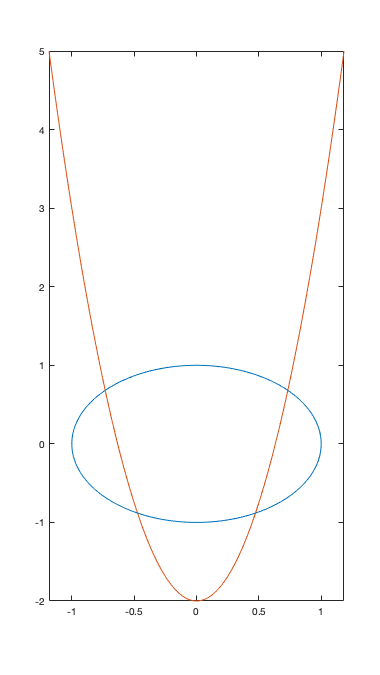
\includegraphics[width=.60\textwidth]{multinewton.png}
      \end{center}
    \end{figure}
    Where these two functions intersect are points where both functions are satisfied, so let's pick our initial values around there. Doing so 
    we get $x_0 = (-.5, -.9)$, $x_0 = (-.7, .7)$, $x_0 = (.5, -.9)$, $x_0 = (.7, .7)$. Using these values as the input to our Newton routine we get, \\
    \textbf{Console:}
    \begin{center}
      \lstinputlisting[basicstyle=\footnotesize]{r4.txt}
    \end{center}
 \end{proof}
\end{exercise}
\vspace{.5in}





\begin{exercise}{2.4} Prove Corollary 6.7. If $x$ is a feasible solution to the primal, $y$ is a feasible solution to the dual, and 
  $c^Tx = b^Ty,$ then $x$ and $y$ are optimal for their respective problems. 
  \begin{proof} Suppose $x$ is a feasible solution to the prime LP problem, $y$ is a feasible solution to the dual LP problem, and 
    $c^Tx = b^Ty$. By Weak Duality we know that for all feasible solutions $h$ in the primal and $g$ in the dual, $c^Th \leq b^Tg$.
    Therefore for all feasible solutions $h$ in the primal we know that $c^Th \leq b^Ty = c^Tx$. So we get that for all feasible solutions
    $h$ in the primal $c^Th \leq c^Tx$ and thus $x$ must be the optimal solution in the primal.


    Similarly, for all feasible solutions $g$ in the dual we get that $b^Tg \geq c^Tx = b^Ty$. So we get $b^Tg \geq b^Ty$ for all feasible solutions 
    $g$ in the dual and thus $y$ must be optimal solution in the dual. 
 \end{proof}
\end{exercise}
\vspace{.5in}




\begin{exercise}{2.8} Using duality theory find the solutions to the following linear programs, 
  \begin{align*}
    \text{Minimize } z = x_1 + 2x_2 + &\dots + nx_n\\
    \text{Subject to } x_1 \geq &1\\
    x_1 + &x_2 \geq 2\\
    &\vdots\\
    x_1 + &x_2 + \dots + x_n \geq n\\
    x_1, &x_2, \dots, x_n \geq 0
  \end{align*}
  \begin{proof} First let's convert the given LP problem into standard form. Doing so we get the following, 
    \begin{align*}
      \text{Minimize } z = x_1 + 2x_2 + &\dots + nx_n + \sum_{i = 1}^n + e_i\\
      \text{Subject to } x_1 + s_1 = &1\\
      x_1 + &x_2 + s_2 = 2\\
      &\vdots\\
      x_1 + &x_2 + \dots + x_n + s_n = n\\
      x_1, &x_2, \dots, x_n, s_1, s_2, \dots, s_n \geq 0
    \end{align*}
    Note that the matrix $A$ that we have formed looks like $A = [L_1 I_n]$ where $L_1$ is a lower triangular matrix with all 
    ones. Generating the dual problem we get the following, and note that $A^T$ now looks like an upper triangular matrix stacked on top of 
    an identity matrix,
    \begin{align*}
      \text{Maximize } w = y_1 + 2y_2 + &\dots + ny_n + \sum_{i = 1}^n + e_i\\
      \text{Subject to } y_1 + &y_2 + \dots + y_n \leq 1\\
      y_2 + y_3 + &\dots + y_n \leq 2\\
      &\vdots\\
      x_n \leq &n\\
      s_1, s_2, &\dots, s_n \leq 1
    \end{align*}
    Now consider the feasible solution in the primal, $x = (n, 0,\dots, 0)$ with excess variables set to zero, which gives a function value of $z = c^Tx = n$. Also consider the 
    feasible solution in the dual, $y = (0, 0, \dots, 1, 0, \dots, 0)$ where the one corresponds to $x_n$ gives us $w = b^Ty = n$. Since we have two feasible solutions in their
    respective problems, that also have the property that $c^Tx = b^Ty$ they must be optimal in their respective problems. Therefore we get that $x = (n, 0,\dots, 0)$ is the optimal solution to 
    the original problem (excess zeroes removed). 
 \end{proof}
\end{exercise}
\vspace{.5in}







\begin{exercise}{2.11} Prove that if the problem $L_1$
  \begin{align*}
    \text{Minimize } z &= c^Tx\\
    \text{Subject to } Ax &= b\\
    x \geq &0
  \end{align*}
  has a finite optimal solution, then the new problem $L_2$
  \begin{align*}
    \text{Minimize } z &= c^Tx\\
    \text{Subject to } Ax &= \hat{b}\\
    x \geq &0
  \end{align*}
  cannot be unbounded for any choice of the vector $\hat{b}$.
  \begin{proof} Suppose for the sake of contradiction that there exists a $\hat{b}$ such that $L_2$ is unbounded. 
    Choose the said $\hat{b}$ and construct the dual of $L_2$, namely $D_2$. Note that the constraints of $D_2$ are denoted by 
    $A^Ty \leq c$. By Corollary 6.6, since $L_2$ is unbounded, we know that $D_2$ is infeasible and by definition there exists no solution for
    $A^Ty \leq c$. Now consider the dual of $L_1$, namely $D_1$ and note that it has the same constraints as $D_2$ i.e  $A^Ty \leq c$. By Strong Duality 
    since $L_1$ has an optimal solution, then $D_1$ also has an optimal solution, $y^*$. Note that since $y^*$ is optimal it must satisfy $A^Ty^* \leq c$. Therefore 
    $y^*$ is also a feasible solution to $D_2$. Thus a contradiction.  
 \end{proof}
\end{exercise}
\vspace{.5in}



\begin{exercise}{Problem P10} Suppose we have an LP problem in standard form, and we do not have a basic feasible solution. 
  Write code which implements the phase-1 strategy for generating an initial basic feasible solution.  
  \begin{proof}[Solution] The following code sets up the new phase one LP problem. We must add the $m$ artificial variables to 
    the matrix $A$ in the form of an $mxm$ identity matrix so our new $A$ looks like $[A I_m]$. The goal is to minimize the artificial variables 
    so we end up with $c = (0, \dots, 0, 1, \dots 1)$ a vector with $n$ zeros followed  by $m$ ones. An initial basic feasible solution can then easily be 
    constructed by $x_0 =(0, \dots, 0, b_1, b_2, \dots, b_m)$. We report that the problem is unbounded if the value of our objective function for the phase one problem 
    is greater than zero.\\
    \textbf{Code:}
    \begin{center}
      \lstinputlisting[basicstyle=\footnotesize]{phaseone.m}
    \end{center}
 \end{proof}
\end{exercise}
\vspace{.5in}



\begin{exercise}{Problem P11} Use the provided scripts to run the simplex method on a Klee-Minty cube of size $n$.
  On your machine how big of an $n$ can you run in under 20 seconds? For this maximum $n$, how many iterations does it take to find the optimal 
  solution? What are the number of constraints and the number of variables if you were to put the problem in standard form?
  \begin{proof}[Solution] On my machine size $n = 13$ took 19.3544 seconds to run, and $n = 14$ took about 60 seconds. 
    For $n = 13$ it took 8192 iterations of the simplex method to find the optimal solution. The Klee-Minty cube as defined in the 
    comments of Klee-Minty.m is an LP problem with $n$ variables, $2n$ inequality constraints. When we transform it into standard form 
    $n$ slack variables are added, so we end up with $2n$ variables, $n$ equality constraints, and $2n$ nonnegativity constraints. 
  \end{proof}
  
\end{exercise}







\end{document}


































